\chapter{The CMS Detector at the LHC}
\label{c:CMS_Detector}

\section{Introduction to the LHC}
\label{s:Introduction}
The Large Hadron Collider (LHC) at the Organisation Europ\'{e}enne pour la Recherche Nucl\'{e}aire (CERN) near
the Swiss city of Geneva was constructed with the aim of investigating various aspects of the Standard Model
of physics. The Standard Model has stood up well to scientific scrutiny for several decades.
However, areas of current interest such as the Higgs mechanism and the role electroweak symmetry breaking
plays in it, and physics beyond the standard model such as supersymmetry (explained in further detail in
Section~\ref{c:the_standard_model}), require the acceleration of particles to high energies (of the order of
TeV). The Compact Muon Solenoid (CMS) general-purpose detector is one of four detectors located around the
LHC, approximately 100~m below ground level. The geographical site and location of the various experiments are
shown in Figure~\ref{fig:LHC_and_CMS_map}.

\begin{figure}[hbtp]
   \centering
     \includegraphics[width=0.35\textwidth]{Chapters/03_Detector/Images/lhc-pho-1997-169.jpg}\\
     \includegraphics[width=\textwidth]{Chapters/03_Detector/Images/0812015.jpg}%\hfill
     \caption{Map of LHC location (top) and schematic of LHC and experiments (bottom). CMS is located at Point
     5 on the LHC ring.}
     \label{fig:LHC_and_CMS_map}
\end{figure}

The 27~km circumference LHC can collide two proton beams, each composed of 2808 bunches, at a design energy of
7~TeV per beam (meaning a 14~TeV centre of mass energy in collisions) with a luminosity of $10^{34}
cm^{-2}s^{-1}$ at a collision rate of 25~ns (40~MHz). In fact, in 2011 the machine ran at a centre of mass
energy of 7~TeV at a bunch spacing of 50~ns (leading to 8 proton-proton interactions per bunch crossing) and
CMS recorded a peak instantaneous luminosity of $3.7\times10^{33}~cm^{-2}s^{-1}$. In 2012 the centre of mass
energy was increased to 8~TeV (21 proton-proton interactions per bunch crossing) and CMS recorded a peak
instantaneous luminosity of $7.7\times10^{33}~cm^{-2}s^{-1}$. The design energy and luminosities mentioned
previously are planned when data taking begins again after Long Shutdown 1 (currently scheduled to be around
May 2015) and after Long Shutdown 2 (in 2019) respectively. $6.1~fb^{-1}$ and $23.3~fb^{-1}$ of data was
delivered to CMS during the 2011 and 2012 data taking periods respectively;
Figure~\ref{fig:integrated_luminosity} shows the increase in integrated luminosities delievered to CMS over
time.

The acceleration process begins with a tank of hydrogen. After stripping electrons off the hydrogen atoms
using an electric field, the remaining protons are inserted into the LINAC2 which accelerates them up to
50~MeV. From here, the proton beam is injected into the Proton Synchrotron Booster (PSB) which increases the
energy to 1.4~GeV, followed by the Proton Synchrotron (PS) which accelerates the beam to 25~GeV and the Super
Proton Synchrotron (SPS) where the beam energy reaches 450~GeV. Finally, the protons are injected into the LHC
where two beampipes carry the beams in a clockwise and an anti-clockwise direction while accelerating them
up to the required collision energy. Filling the LHC rings takes approximately 4 minutes, followed by
approximately 20 minutes until the beams reach energies of 4~TeV (during 2012 data taking). Once the collision
energies have been attained, the counter-circulating beams are brought to collide at the four main LHC
experiments CMS, ATLAS, LHCb and ALICE. ALICE is specifically designed to investigate heavy ion collisions
(as opposed to protons), while LHCb investigates b-meson physics.

\begin{figure}[hbtp]
   \centering
     \includegraphics[width=0.75\textwidth]{Chapters/03_Detector/Images/int_lumi_cumulative_pp_2.png}\\
     \caption{Cumulative luminosity delivered to CMS over time during 2010, 2011 and 2012 proton-proton data
     taking periods.}
     \label{fig:integrated_luminosity}
\end{figure}

\section{Overview of CMS}
\label{s:Overview}
Compact Muon Solenoid is both the name of one of the detectors at the LHC, and of the collaboration of
people worldwide who work to build, operate, maintain and upgrade it and to analyse the data recorded from it.

CMS is a general-purpose detector, designed to be efficient at detecting new physics with a wide range of
signals. The detector measures 14.6~m in diameter, 21.6~m in length and weighs 12500~tonnes
\cite{CMS_experiment}. In general, the different components of CMS are arranged in concentric layers around
the interaction point in the beam pipe, which is the point at which the two beams of proton bunches collide
\ref{fig:CMS_diagram}. As the products of any collisions that occur in the bunch crossing travel outwards from
the interaction point, they pass through the various sub-detectors leaving signals as they do so. A subset of
the information from some sub-detectors (the calorimeters and muon chambers, described in
Section~\ref{s:Subdetectors}) is then processed by a trigger while information from other sub-detectors is
buffered on the detector.

\begin{figure}[hbtp]
   \centering
     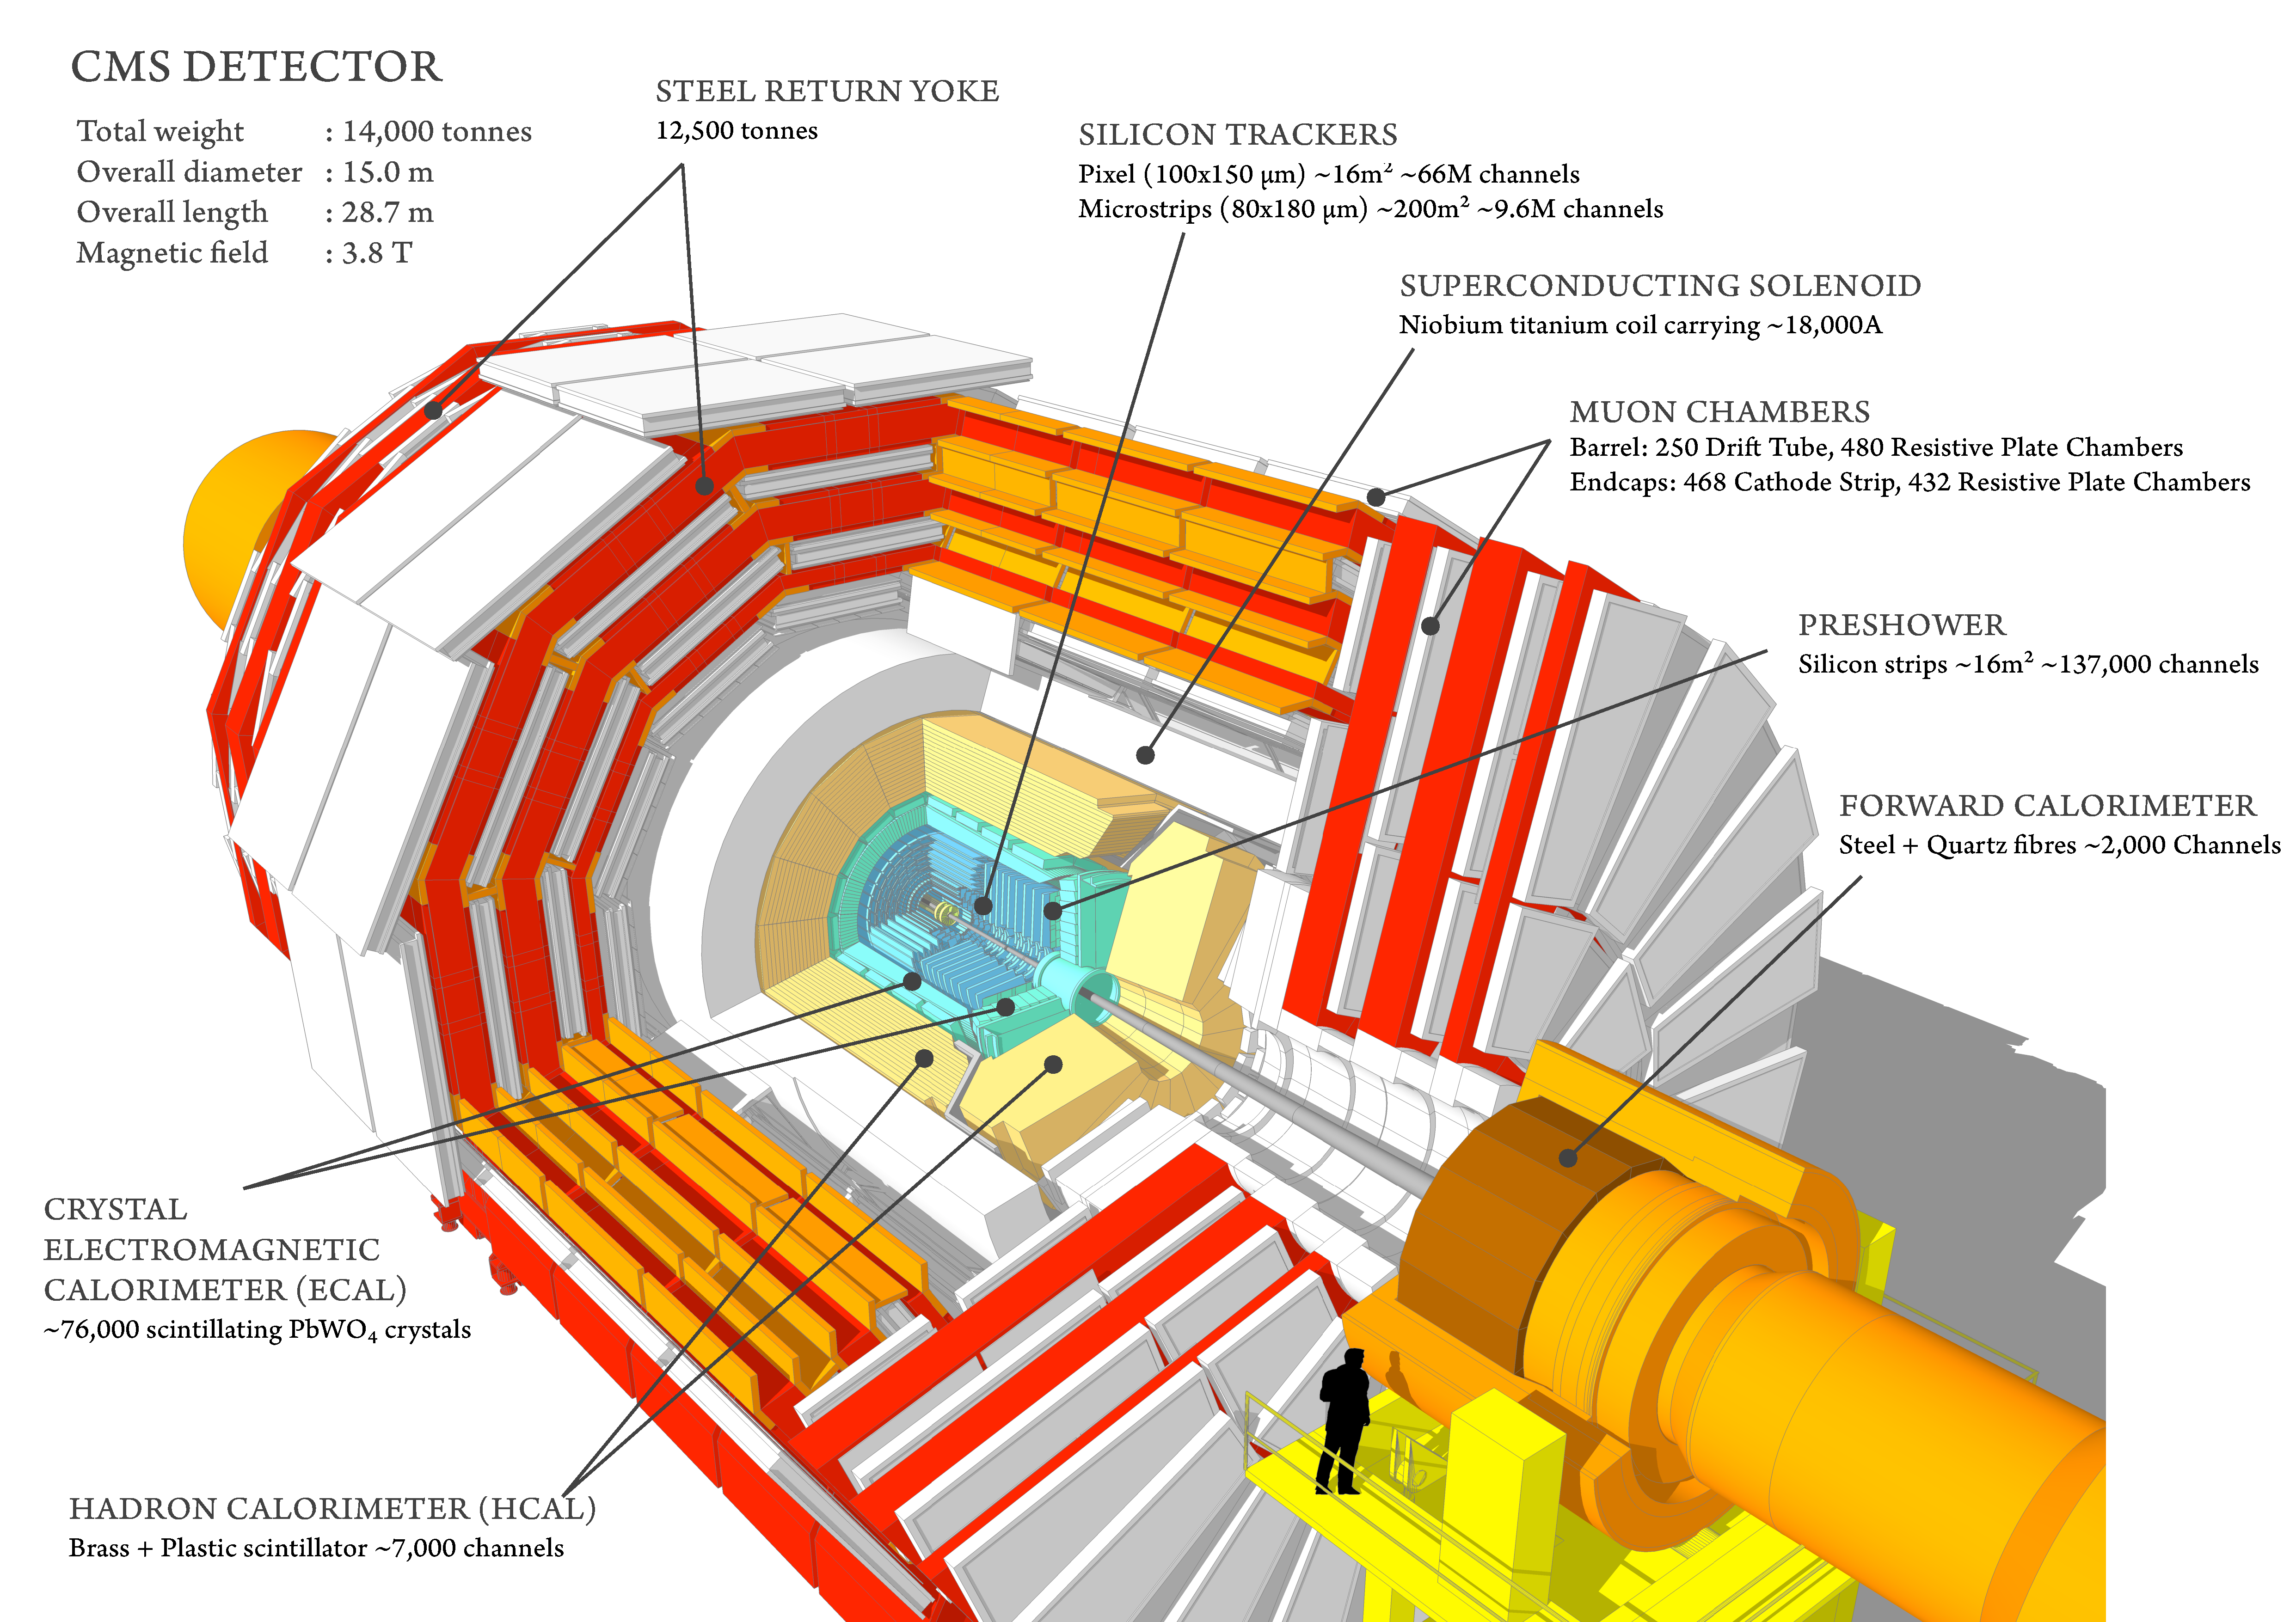
\includegraphics[width=\textwidth]{Chapters/03_Detector/Images/cms_120918_02.pdf}\hfill
     \caption{Diagrammatic sectional view of the CMS detector \cite{Sakuma_sketchup}}
     \label{fig:CMS_diagram}
 \end{figure}

The design of CMS is based firstly around a superconducting solenoid magnet. Around and inside ths magnet are
the pixel and strip tracker, the electromagnetic calorimeter, the hadronic calorimeter, the return yoke for
the magnet and the muon detectors. The coordinate system of the detector is designated with the origin as the
intersection point of the two beams in the beam pipe, with the x-axis positive towards the centre of the LHC
ring, with the y-axis positive vertically upwards and with the z-axis pointing along the beampipe in an
anticlockwise direction. The angle $\phi$ is defined as the angle in the x-y plane, transverse to the beampipe
starting from the x-axis. $\theta$, the polar angle is defined as the angle in the z-y plane starting from the
z-axis (the beampipe). $\theta$ is related to the pseudorapidity, $\eta$, by the formula
$\eta$=-ln(tan($\theta$/2)), so that $\eta$ ranges from 0 at $\theta$ = 90$^{\circ}$ to $\infty$ at $\theta$ =
0 $^{\circ}$ \cite{CMS_TDR1}. The two ends of the detector, at high $\eta$ values, are called the endcap regions while the
central area at lower $\eta$ values is called the barrel region.

\section{Sub-Detectors}
\label{s:Subdetectors}

\subsection{Tracker}
\label{ss:Tracker}

Each event that is recorded in the CMS detector is one crossing of the bunches of protons of which the beams
are comprised. Any charged particles produced as a result of the proton-proton collisions in these bunch
crossings need to be recorded for later use in reconstruction of particle information such as trajectories and
charges. This is achieved using the tracker section of CMS which consists of silicon sensors in two forms:
pixels and strips. As the charged particles travel through these silicon sensors, electron-hole pairs are
produced in the silicon which are processed by readout chips. This readout is carried out by the
Analogue Pipeline Voltage (APV) chip (a new chip called the CMS Binary Chip (CBC) is intended to replace
the APV in the HL-LHC after Long Shutdown 3, which is currently scheduled for 2023-2024).

The purpose of the tracker within the CMS detector is to track the trajectory of charged particles as they
travel out from the interaction point. The tracker is split into two parts, with an inner silicon pixel
detector and an outer silicon strip detector. The inner pixel detector consists of three layers in the
barrel region at distances of 4.4~cm, 7.3~cm and 10.2~cm from the beam line with two endcap discs at each end.
Each pixel measures 100~$\mu m$ by 150~$\mu m$ and the entire pixel detector covers an area of only
approximately $1~m^{2}$ but contains 66~million pixels in total.

The strip tracker is comprised of ten layers in the barrel region at distances ranging from 20~cm to 1.1~m
from the beam pipe. The four inner layers (at distances of 26~cm, 34~cm, 42~cm and 50~cm from the beampipe)
are collectively named the Tracker Inner Barrel (TIB), while the outer six layers (at distances of 61~cm,
70~cm, 78~cm, 87~cm, 97~cm and 108~cm from the beampipe) are known as the Tracker Outer Barrel (TOB). The
endcaps consist of twelve discs, three of which correspond to the Tracker Inner Discs (TID) at z-distances
from 75~cm to 100~cm, and nine to the Tracker End Caps (TEC) at z-distances between 120~cm and 280~cm
\cite{Palmonari:1260970}. A diagrammatic view of the CMS tracker, including both pixels and strips, is shown
in Figure~\ref{fig:CMS_strip_tracker}. The largest silicon detector ever constructed, the strip tracker
contains about ten million channels and covers an area of approximately $200~m^{2}$
\cite{CMS_experiment,CMS_TDR1}. The operating temperature of the tracker during 2011 and 2012 has been
0~$^{\circ}$C for the pixels and +4~$^{\circ}$C for the strips but will be lowered for both after Long
Shutdown 1 \cite{Butz:1497745}.

\begin{figure}[hbtp]
   \centering
     \includegraphics[width=\textwidth]{Chapters/03_Detector/Images/tracker.pdf}\hfill
     \caption{Cross-sectional diagram of the CMS strip tracker; each line represents a detector module
     \cite{CMS_TDR1}}
     \label{fig:CMS_strip_tracker}
\end{figure}

As a charged particle passes through the various layers of silicon in these detectors, electrical signals are
created which are then read by readout electronics. Offline algorithms then use the data relating to which
strips and sensors received 'hits' to reconstruct the tracks of charged particles and this information is
later used for particle reconstruction and identification \cite{CMS_experiment,CMS_Tracking_Early_Results}.

Neutral particles could also leave signals in the tracker in a small proportion of cases if the particle
interacts with a silicon atom and/or converts to charged particles such as a photon conversion to two
electrons. In the majority of cases, the presence of neutral particles must be detected from their energy
deposits in the calorimeters.
For physics analyses, the premise employed is that the curving of particle tracks within a magnetic field
allows the calculation of the particle momentum and charge. An important requirement of the tracker is that it
must allow the above whilst not affecting the energy of the particle being tracked. The silicon in the tracker
sensors also does not stop particles, thereby allowing them to pass through this innermost layer of the
detector and interact with outer layers.

%With the higher data rate expected after the LHC upgrades over the coming decade,
%pile-up will become an important issue, with approximately 20 interactions per bunch crossing even at the
%current design luminosity. This number is expected to increase to 100-200 following Long Shutdown 3.

The tracker readout chips must be able to distinguish from which bunch crossing a particle was produced
(bunch-crossing identification).
%At higher luminosities, the occupancy (the fraction of channels with a 'hit') increases,
%which makes pattern recognition more difficult for track reconstruction algorithms and readout systems. The
%higher tracker resolution desirable for such circumstances also requires more sensors and readout chips. As a
%result, any new chip would need to be more efficient in its use of power whilst processing the data and/or
%require the associated cooling systems to be more efficient. Indeed, studies have shown that the present
%tracker could itself produce acceptable tracking performance in such conditions based on simulations of
%heavy-ion collisions, which produce similar numbers of tracks per event to that expected after the luminosity
%upgrades at the LHC [10].

%The LHC upgrades are split into 2 phases. The pixel detector will be upgraded during Phase 1, and will be an
%on-going process during both Long Shutdown 1, Long Shutdown 2 and shorter intermediate shutdowns. The strip
%detector will be upgraded during Phase 2, more specifically during Long Shutdown 3 [11][12].

The required tracker characteristics of high granularity, good resolution, fast response to process the high
data rate without losing potentially valuable information, radiation hardness and keeping detector material to
a minimum to minimise interactions of the particles with detector matter, resulted in silicon being chosen to
construct the tracker. One of the advantages of using silicon over gaseous detectors is that silicon produces
more charge carriers per unit of length travelled by a particle. This therefore means the silicon thickness
can be reduced, typically around 300~$\mu m$ per layer. Silicon also allows fast signal transfer, of the order
of about 10~ns, as the aforementioned charge carriers travel quickly through silicon.
Furthermore, the spacing between strips in a silicon sensor, known as the strip pitch, can be manufactured to
be extremely small, down to the order of around 10~$\mu m$.
The silicon sensors that make up the strip tracker in the CMS detector vary in thickness depending on their
location. Sensors of 320~$\mu m$ thickness are utilised in the TIB and TID, 500~$/mu m$ in the TOB, and a
mixture of both thicknesses is used in the TEC. The strip pitches and their lengths vary such that there are
fifteen distinct types of sensor geometries in the strip tracker
\cite{Commissioning_and_Performance_Strip_Tracker}. Thicker sensors are used in the outer sections of the
strip tracker in order to maintain a high signal to noise ratio, since the increased strip lengths in this
region lead to increased electronics noise due to higher capacitance \cite{CMS_experiment}.
Furthermore, in general the occupancy needs to be low (the fraction of channels with a hit in an event was
desired to be 1~\% or lower at the nominal LHC luminosity) so that pattern recognition can be carried out
efficiently and so the amount of simultaneous data to be read out is manageable. In order to maintain a low
occupancy, a high granularity is maintained in the strip tracker with strip lengths less than 20~cm and strip
pitches less than 205~$\mu m$ \cite{Palmonari:1260970}.
While high granularity is beneficial for high precision tracking, it also results in a high number of
channels, which in turn requires large amounts of electronics for readout and leads to high heat load.

On a global scale, the tracker data is read out using a combination of interoperating systems.
The data from the Analogue Pipeline Voltage (APV25) tracker readout chips is taken via optical fibres to 440
off-detector Front End Drivers (FEDs) (which make up 63\% of the total number of FEDs in CMS).
The FEDs then forward the data to the online Data Acquisition System (DAQ). In addition, off-detector Front
End Controllers (FECs) control the front-end electronics by means of approximately 350 control rings,
including triggers, clock and monitoring \cite{CMS_experiment, Corrin}.

%As a result of the higher collision rates to be expected after
%these upgrades, the CMS tracker will require an improvement in its infrastructure because of radiation damage
%it will have suffered by that point and to ensure that it is robust enough to handle the higher levels of
%radiation after the upgrades. The pile-up is also expected to be in the range of 100 to 200 interactions per
%bunch crossing which also necessitates an improvement in the CMS tracker performance in order to ensure
%valuable data are not lost during collisions \cite{CMS_Silicon_Tracker_upgrade_for_HL-LHC}.

% Within the lattice of pure silicon, there are well-defined bands of energy levels called the conduction band
% and the valence band. The band gap is the difference in energy between these two bands and varies depending on
% the material. At absolute zero, -273$^{\circ}$C, almost all the electrons can be said to be fixed in place in
% this lattice in the valence band, meaning that if an electric field is applied across the silicon, no current
% would be able to flow. When energy is input to the system and an electron gains energy, it may be able to
% cross the band gap to the conduction band, in which case a hole would be present in its previous place in the
% valence band. At this point, both the electron and the hole are mobile and can move freely in current flow,
% for example, under the influence of an electric potential. Materials with a large band gap are insulators, and
% those with a small band gap (or even sometimes with energy bands that overlap with each other) are conductors.
% Silicon, being a semiconductor, has a 'medium' sized band gap of approximately 1.12eV. Nevertheless, the
% number of mobile electrons, above absolute zero, is still large enough to make it difficult to distinguish the
% real signal from the inherent noise in the silicon, known as leakage current (explained in Section 2.3.2).
% In order to decrease this number of free electrons and holes in silicon to obtain a much cleaner signal from a
% traversing particle (i.e. improve the signal to noise ratio), a process called doping is employed to increase
% the number of charge carriers. This involves the substituting of silicon atoms in the lattice with atoms of
% other elements like arsenic, phosphorous, boron or aluminium. In the case of the former two, both have five
% valence electrons. Four of these electrons bond to the four valence electrons present in a silicon atom,
% leaving one electron that can be easily removed from the lattice to the conduction band. This 'donation' of
% electrons to the conduction band increases the number of charge carriers. This type of silicon is called
% n-type silicon because the additional charge carriers are negative. Similarly, if boron or aluminium atoms are
% introduced to the silicon lattice, their three valence electrons bond to the electrons in a silicon atom but
% one silicon electron has nothing to bond to, creating a mobile positive hole. The addition of holes (which
% 'accept' electrons) leads to this type of silicon being called p-type because the additional charge carriers
% are positive.
% Although both p- and n-type silicon increase the number of free charge carriers, a PN-junction can be created
% by attaching a piece of n-type silicon to a piece of p-type silicon. Considering a PN-junction in isolation,
% mobile electrons from the n-type silicon would diffuse into the p-type silicon and unite with the holes from
% the p-type material, leaving behind the positively charged donor atoms. Similarly, the mobile holes from the
% p-type silicon would diffuse to the n-type silicon and leave behind negatively charged acceptor atoms. As
% these electrons and holes move to the two sides of the junction, the resulting electric field opposes the
% initial diffusion of electrons and holes, eventually reaching a state of equilibrium. Once equilibrium is
% reached, this area around the PN-junction will contain no mobile charge carriers and is called the depletion
% region.
% However, if a reverse bias voltage is applied to the silicon (a negative terminal connected to the p-type
% silicon and a positive terminal to the n-type silicon), then the electrons from the n-type silicon, rather
% than diffusing towards the junction, will be attracted towards the positive terminal. Similarly, the holes
% from the p-type silicon will be attracted towards the negative terminal, as shown in Figure 7.
% 
%  
% A higher reverse bias voltage leads to a larger depletion width as more electrons and holes are carried away
% from the junction. At high enough voltages, the width of the depletion region can be made equal to the width
% of the silicon; this voltage is known as the depletion voltage. At this stage, there are no free charge
% carriers anywhere in the silicon and it is in this state that silicon detectors are operated, thus ensuring
% that any charge carriers are only produced as a charged particle travels through the silicon. In this state,
% silicon detectors are effectively reverse biased diodes, only allowing a current to flow in one direction.
 
%Figure 8 - Basic diagram of silicon strip detector with p+ strips (green) on n-bulk (blue) [24].

% The silicon sensors in the CMS strip tracker are p+ strips (which denotes a high concentration of p-type
% impurities) on n-bulk sensors, similar to the diagram in Figure 8. As the silicon is ionised by a traversing
% particle, mobile charge carriers are created which then travel, due to the depletion voltage, to the p+ strips
% (holes) or to the backplane (electrons). As the signal will be created on a particular strip (or strips), it
% will then be possible to deduce the position of the particle.

% 2.3.2 Radiation Hardness The current tracker front-end electronics were initially designed to last about 10
% years in operation under the radiation conditions of the detector [5]. The higher radiation they will be
% subjected to as a result of the higher luminosity and higher collision energies at the HL-LHC will clearly
% impose the requirement that all components, including sensors and electronics, should be manufactured to a
% higher standard of radiation hardness. Radiation damage can occur when particles of high enough energy are
% created in the collisions at the centre of CMS that when they pass through the silicon tracker, they collide
% with atoms in the lattice. This damage is done most often by neutrons, in particular low energy neutrons from
% calorimeters and other detector elements, which interact with nuclei in the silicon and move atoms out of
% place. These atoms are knocked out of place into levels where there is usually no atom, known as interstitial
% levels. An energy of around 15eV is necessary for this to happen; generally at energies of 2keV or less only
% isolated displacements occur, whereas for energies between 2 and 12keV, one or more defect clusters will be
% created. The removal of donor atoms in this way leads to a change in the doping concentrations and eventually
% to an increase in the leakage current (current which may flow when there is no ionising particle traversing
% the silicon). A leakage current will in turn require a higher depletion voltage to remove additional electrons
% or holes captured by the electronically active defects.
% The leakage current is temperature dependent and can be mitigated by using low temperatures. The planned
% running temperature of the CMS silicon tracker in the HL-LHC is planned to be lowered from +4$^{\circ}$C to
% the region of -20$^{\circ}$C to -40$^{\circ}$C due to the benefits in terms of radiation damage. To evaluate
% the behaviour of the proposed CBC in these conditions, an environmental chamber was used to carry out tests at
% varying temperatures in this project. If a leakage current is present, this will lead to noise in the system,
% since current will always flow and any signal would sit on top of this noise. If subject to high levels of
% radiation damage, the leakage current increases to levels at which excessive amounts of power are dissipated,
% and the noise in the readout will be too high to read a clean signal.
% 
% 2.3.3 Noise The aforementioned leakage current is a result of the quantised nature of the charge carriers.
% This noise is present even when there is no signal present, and increases as radiation damage increases the
% leakage current.
% Other potential sources of noise include electronic noise caused by thermal fluctuations of the charge
% carriers. This would manifest as noise in the amplifier at the front end of the CBC and would increase
% proportionally with the capacitance of the connected input system [25]. Another contributor to noise in the
% system could be from non-linearity of the analogue to digital converter (ADC) in the CBC that converts the
% incoming analogue pulse to a digital signal [25].
% The dominant source of noise in our test system is likely to have resulted from electronic noise in the
% connected laboratory setup. In practice, the external noise under operational conditions when the CBC is
% connected to the CMS detector should ideally be maintained lower than the noise in the amplifier.


\subsection{Electromagnetic Calorimeter}
\label{ss:Ecal}
The electromagnetic calorimeter, often referred to as the ECAL, is a hermetic, homogeneous
subdetector constructed of scintillating crystals of lead tungstate ($PbWO_{4}$), and is the next layer
outside the tracker. Any electromagnetic particles such as electrons or photons are absorbed by the ECAL
crystals. The energy of the particles is absorbed by the crystals which then scintillate emitting a blue-green
coloured light. These signals are then detected by connected photodetectors and processed by readout
electronics.

The high density crystals used ($8.28~g/cm^{3}$), short radiation length ($X_{0} = 0.89cm$) and small
Moli\`{e}re radius of 2.2~cm (EXPLAIN THIS? OR REMOVE IT?) lead to a compact calorimeter with fast response
time, high granularity and of course capable of withstanding the radiation levels within CMS. The barrel
region of the ECAL consists of 61,200 crystals and extends up to a pseudorapidity, $\eta\pm1.479$. Each
individual barrel crystal is $25.8X_{0}$ thick and has cross-sectional dimensions of $22~\times~22~mm^{2}$,
which equates to $0.0174~\times~0.0174$ in the $\eta-\phi$ plane.These crystals are divided into 36
supermodules, with each consisting of 4 modules. The endcaps are comprised of 7,324 crystals, cover the range
$1.479\leq\eta\leq3.0$ and are split into two halves known as ``Dees" and is divided into operating segments
of $40^{\circ}$ each. The endcap crystals have slightly larger dimensions, having a thickness of $24.7X_{0}$
and cross-sectional dimensions of $28.62~\times~28.62~mm^{2}$ \cite{CMS_experiment,ECAL_frontend_monitoring}.
Figure~\ref{fig:CMS_ECAL} shows the layout of the ECAL.

The signals in the crystals are collected by avalanche photodiodes in the barrel region and vacuum
phototriodes in the endcaps. The numbers of photoelectrons produced is dependent on temperature, with
increasing temperature resulting in a decrease in the number of electrons at a rate of
$-3.8\pm0.4\%/^{\circ}C$. A cooling system is thus employed which maintains a stable operating temperature of
the ECAL system to within $\pm0.05^{\circ}C$, with a nominal operating temperature of $18^{\circ}C$
\cite{CMS_experiment}. The energy resolution of the ECAL has been shown to follow $\sigma_{E}/E =
2.8\%/\sqrt{E}\oplus 12\%/E \oplus 0.3\%$ where the three constant terms come from stochastic fluctations such
as photostatistics, electronics noise and temperature stability and calibration uncertainties
\cite{ECAL_calibration_and_resolution_at_7TeV}.

\begin{figure}[hbtp]
   \centering
     \includegraphics[width=0.7\textwidth]{Chapters/03_Detector/Images/ECAL.pdf}\hfill
     \caption{Diagram of the ECAL showing barrel supermodules, endcaps and preshower detectors.
     \cite{ECAL_calibration_and_resolution_at_7TeV}}
     \label{fig:CMS_ECAL}
\end{figure}

\subsection{Hadronic Calorimeter}
\label{ss:Hcal}
The next subdetector outside the ECAL is the hadronic calorimeter (HCAL) which works in a similar way to
the ECAL, in this case by absorbing hadron jets. The HCAL is located at a distance of 1.77~m to 2.95~m from
the beamline, with an additional outer hadronic calorimeter also installed outside the magnet due to
radial restrictions imposed by the magnet coil. The HCAL barrel (HB), outer (HO) and endcaps (HE) cover
the $\eta$ range up to 3.0, with the forward HCAL (HF) placed at $\eta$ up to 5.2 increasing the coverage.
Figure~\ref{fig:CMS_HCAL} shows the a quarter of the HCAL endcap.


The HB
The HCAL is a sampling calorimeter, meaning it is composed of alternating absorber layers (made of brass) and
scintillator layers (made of plastic). A hadronic particle produces a shower of secondary particles when it
strikes an absorber layer; this process is repeated as these secondary particles themselves pass through
successive absorber layers. The scintillator layers in between absorb the energy of these particles, emitting
light as they do which is fed to readout electronics via optical fibres to measure the particle energies. 



\begin{figure}[hbtp]
   \centering
     \includegraphics[width=\textwidth]{Chapters/03_Detector/Images/HCAL.pdf}\hfill
     \caption{A longitudinal schematic of the HCAL showing the location of the hadron barrel (HB), endcap
     (HE), outer (HO) and forward (HF) calorimeters \cite{CMS_experiment}}
     \label{fig:CMS_HCAL}
\end{figure} 

\subsection{Superconducting Magnet}
\label{ss:Magnet}
The magnet of the CMS detector is the largest and highest field strength superconducting solenoid ever
constructed. It can produce a magnetic field up to 4~T (a field strength of 3.8~T is used in running) with a
stored energy of 2.7~GJ \cite{CMS_TDR1}. The cold bore, cooled to 4.5~K using liquid helium, has dimensions of
12.5~m length and 6~m diameter, and weighs 220~tonnes \cite{Cryogenic_System_for_Superconducting_Solenoid}.
Due to design constraints and structural requirements, the magnet itself provides some of the structural strength both to support itself and to
withstand its own magnetic bursting force on the coil \cite{CMS_experiment}.

\begin{figure}[hbtp]
   \centering
     \includegraphics[width=0.5\textwidth]{Chapters/03_Detector/Images/Cold_mass.png}\hfill
     \caption{Bore of the CMS solenoid magnet in vertical position in the CMS assembly hall, SX5, prior to
     installation \cite{CMS_experiment}}
     \label{fig:CMS_magnet_cold_bore}
\end{figure}
 
The cold bore, pictured in Figure~\ref{fig:CMS_magnet_cold_bore} in the CMS assembly hall, is enclosed in a
steel return yoke weighing 10,000~tonnes with the aim of containing and returning the magnetic field. The yoke is interspersed in the
muon chambers and is made up of 5 barrel segments and 6 endcap discs. The magnet was designed in a manner such
as to facilitate assembly at ground level prior to lowering into the CMS experimental cavern, UX5.
Despite the challenges involved in constructing such a powerful magnet, the high track-curving power created
by the high magnetic field was desirable in order to provide good momentum resolution of the tracking
components.

\subsection{Muon Chambers}
\label{ss:Muon_Chambers}
Muons pass through all the previous inner sub-detectors, losing very little energy as they traverse them
(around 1~MeV/mm), leading to the muon chambers being located outermost in the detector. There are, in fact,
three types of muon detectors in use in CMS. The endcaps contain Cathode Strip Chambers (CSCs), the central
barrel regions contain Drift Tubes (DTs), and both regions are reinforced with Resistive Plate Chambers
(RPCs). These systems, in combination with the silicon tracker, are used to determine the momentum of muons by
taking advantage of their curved tracks due to the magnetic field. The different technologies are used due to
the different numbers of particles expected in different areas of the detector and because of technological
considerations regarding the physical areas to be covered \cite{CMS_TDR1}.
Figure~\ref{fig:CMS_muon_system} shows a diagrammatic representation of one quarter of the CMS muon detectors.
The CSCs are used in the endcaps to cover $|\eta|$ values between 1.2 and 2.4 that experience high muon rates
and where the magnetic field of the solenoid is high \cite{CMS_TDR1}. They take the form of four disc layers
each made of 2 (inner layer) or 3 (outer 3 layers) concentric rings. They consist of volumes of gas in which
are found positively charged wires placed at right angles to negatively charged copper strips. To relate these
to the name given to these detectors, the positive wires are the anodes and the negative strips are the
cathodes. As a charged particle passes through the gas it ionises gas atoms and the electrons that are knocked
out travel towards the anode wires. At the same time the resulting positively charged ions in the gas travel
towards the cathode strips. Since the wires and strips are at right angles to each other, the CSCs provide two
position co-ordinates for the passing muon. The CSC detection mechanism is a fast process so their signals are
used for muon triggering \cite{CMS_experiment}.
 
\begin{figure}[hbtp]
   \centering
     \includegraphics[width=0.65\textwidth]{Chapters/03_Detector/Images/MuonSys-mod3.png}\hfill
     \caption{Schematic representation of a quarter of the CMS muon system \cite{Muon_tracking}}
     \label{fig:CMS_muon_system}
\end{figure}

The barrel region DTs cover $|\eta|$ values of less than 1.2, that encounter low rates of low transverse
momentum muons \cite{CMS_TDR1}. They are arranged in four cylindrical layers among the layers of the magnet's
iron return yoke and RPC layers. The layers are slightly staggered to ensure that even a muon of high
transverse momentum will be detected by at least three of the four layers. The drift tubes are gas tubes
containing a stretched wire and enclosed by aluminium plates. As a particle with a charge traverses the volume
of gas, atoms in the gas are ionised and the resulting free electrons travel along electric field lines
towards the positively charged wire. By using the position of the electron along the wire and the time taken
for the wire to detect the electron, two coordinates of the muon position can be deduced.
In comparison to the DTs and CSCs, the RPCs that complement them provide a better resolution in terms of time
(1ns) but a worse resolution in terms of position, and so provide additional trigger information. As their
name suggests, they are constructed of plates, one negatively charged (cathode) and one positively charged
(anode) and made of a plastic with high resistance. In a similar process to the other muon detectors, a gas
that makes up the volume in between the plates is ionised by a passing charged muon. The resulting electrons
create an avalanche of electrons by, in turn, ionising other gas atoms; this avalanche of electrons moves
towards the anode and metal readout strips outside the plastic anode detect the signal for readout. The hit
strips pattern allows a calculation of the muon momentum which is then fed to trigger algorithms.

Neutrinos, like muons, also pass through all the layers of the detector, but cannot be detected directly and
their presence must therefore be deduced by the presence of missing energy in the transverse plane
(perpendicular to the beam directions).

\subsection{Trigger and Data Acquisition}
\label{ss:Trigger}
The data acquisition system (DAQ) is the name given to the combination of the trigger and data recording
systems. At the design bunch crossing frequency of 40~MHz and at the design luminosity of $10^{34}~cm-2s-1$,
the expected number of proton-proton collisions per second is approximately $10^{9}$, translating to 21
proton-proton collisions per bunch crossing on average. Each bunch crossing produces approximately 1~MB of
data, leading to 40,000~GB/s of data. This extremely large amount of data, which is impractical to
record, means that a trigger system is required to filter the events in order to record only data that are of
interest for physics analyses.

There are two levels to the CMS trigger, named Level 1 Trigger (L1) and High Level Trigger (HLT). These work
in sequence with the electronics and readout systems in place in the detector to filter the events to a
practically manageable amount for processing. In combination, these triggers reduce the data rate by at least
a factor of $10^{6}$ \cite{CMS_experiment}.

The L1 Trigger is a pipelined deadtimeless system comprised of calorimeter triggers, muon triggers and a
global trigger that works on a combination of data from the former two. The decisions made by the L1 Trigger
are carried out by 'custom hardware processors', such as Field Programmable Gate Arrays (FPGAs). The data from
a bunch crossing are held in pipeline buffers in the electronics at the front end whilst the information for
the triggers is processed in the CMS service cavern (USC) and the decisions transmitted back to the front end.
The maximum time allowed for this process for each event is 3.2~$\mu s$, which is the time taken for the
signals to be transmitted via optical fibres from the detector to the processors and back again, known as the
latency \cite{CMS_TDR1}. The L1 Trigger outputs data to the HLT at a rate of 100~kHz \cite{CMS_experiment}.

As already mentioned, the trigger uses calorimeter and muon chamber data to reach a decision on an event
within the required timeframe. Tracker data are not currently used since track reconstruction exceeds the
amount of time allowed for the L1 trigger decision. Good trigger performance is related to the quality of the
calorimeters and muon systems. Factors such as good momentum resolution of high momentum muons, good charge
determination of muons, good ECAL energy resolution and good missing transverse energy resolution are required
for the trigger to select interesting events. The trigger was designed as described in order to allow the CMS
experiment to meet the goals of the LHC physics programme \cite{CMS_experiment}.

Unlike the Level 1 Trigger, the High Level Trigger is software-based and run offline in separate processor
farms \cite{CMS_TDR1}. If the Level 1 produces an accept decision, the data which was stored in buffers in the
front end electronics is read into readout buffers from where the DAQ system accesses it. The L1 output rate
of 100~kHz corresponds to a data rate of approximately 100~GB/s. The software making up the HLT processes
these events in a computer farm that carries out fast processing of offline algorithms such as selections and
object reconstructions to reduce the rate down to approximately 100~Hz. This accepted data are then stored on
tape.

All sub-detector readout systems consist of front-end systems into which data is fed from the detector.
When the L1 trigger accepts an event, the data corresponding to that event is extracted from these front-end
buffers and front-end drivers (FEDs) enters the DAQ system. A more detailed description of the DAQ system can
be found in \cite{CMS_experiment} and \cite{CMS_TDR1}.

\section{CMS Computing}
\label{s:CMS_computing}

The CMS offline computing takes on the workload of transferring accepted data from the triggers to both
permanent and temporary storage, and the processing of this data for subsequent analysis, in addition to the
production of simulated CMS data. The resources needed to process the high volumes of data involved require a
distributed computing system; the Worldwide LHC Computing Grid (WLCG) infrastructure, an international
collaboration of LHC experiments and computing centres, is employed to carried out these tasks.

The CMS computing resources are primarily divided into three tiers. Tier 0 (T0) consists of only one site, at
CERN itself. The T0 centre has as its main aims to take accepted data from the detector and transfer it to
permanent storage on tape. Tier 0 computing is also responsible for reconstructing the RAW data into RECO data
formats (see Section~\ref{s:object_reconstruction_and_identification} for more details on data formats). From
the T0 centre, the copies of the data in RECO and RAW format is transferred to T1 centres around the world
(there is also a Tier 1 (T1) centre at CERN, known as the CERN computing centre). Owing to its important role
in ensuring the robust transfer of RAW and RECO data, the T0 resources are not available for analysis by CMS
users. There are seven Tier 1 centres located in various countries within the CMS collaboration. In the UK,
the T1 centre is located at the Rutherford Appleton Laboratory in Harwell, near Oxford. T1 centres provide
reliable computing resources for data storage and processing; RAW data is spread between them, providing a
second copy of the RAW data stored at CERN. The second reconstruction step is also carried out at T1 centres,
in addition to the production of simulated data. These can then be provided to any of the Tier 2 centres at
CMS institutes (typically universities) where they may be temporarily stored. Typically, T2 centres are used
to run users' final analyses and produce simulations \cite{CMS_experiment,CMS_TDR1}.

\section{Event Data Model}
\label{s:Event_Data_Model}
Reconstructed data from CMS uses a data model based around an event, called the Event Data Model (EDM), where
one event is one crossing of proton bunches at the centre of CMS which passes the triggers. This model
is created and manipulated within a CMS software framework ( - ADD REFERENCE?) written in C++, with the event
and related objects in the object oriented data analysis framework ROOT.

Everything in an event is passed through a sequence of framework modules to produce subsequent versions of the
data. The arrangement of these data takes the form of layers, with the first of these being RAW. This level
contains the full information from the event in CMS and occupies approximately 1.5-2~MB/event. More
information than is necessary for user analyses is included at this level, and so the majority of CMS users
will not use this data format. Reconstructed level data (RECO) is slightly smaller in size (approximately
0.5~MB/event) and is essentially a compressed subset of the RAW data after modules performing
reconstruction have been run. These modules produce physics objects (like electrons and jets) using algorithms
to reconstruct tracks in the silicon tracker, clusters of deposits in the calorimeters, primary and secondary
vertices, determine particle identification and to correct for detector characteristics such as
non-functioning components.

The third level, Analysis Object Data (AOD), is the smallest of the data formats, requiring approximately
100~kB/event, which is small enough to allow the entire AOD data to be stored at computing centres worldwide.
AOD format is a subset of the RECO data, and is produced by performing a skim on RECO leaving only high level
physics objects (e.g. electrons, jets) which is adequate for most physics analyses. 

In the different cross section analysis presented in this thesis, as in the majority of CMS physics analyses,
this AOD data is processed using the Bristol Top Group's NTupleProduction code (REFERENCE TO NTT CODE ON
GITHUB) to produce private ntuples which are yet again smaller in size, at approximately 3~kB/event. These
ntuples are then converted to simple ROOT histogram files after applying the required selections and
corrections in the BristolAnalysisTools (REFERENCE TO BAT CODE ON GITHUB). Scripts written in Python in
DailyPythonScripts (REFERENCE TO DPS CODE ON GITHUB) are then used to produce final plots and tables.

\section{Upgrades}
\label{s:Upgrades}
It is worth noting at this point, that the CMS experiment, along with the LHC and the other detectors are in a
long term programme of upgrades and maintenance. By 2023 the luminosity provided by the LHC is expected to be
$2\times10^{34}cm^{-2}s^{-1}$ \cite{Technical_Proposal_Upgrade_of_CMS_Detector_through_2020}. The various runs
and shutdowns until 2023 are collectively referred to as Phase 1. In phase 2, or after 2023, long shutdown 3 is
also planned to bring further improvements and upgrades to the performance of the LHC, after which the
luminosity of the LHC is expected to reach $5\times10^{34}cm^{-2}s^{-1}$. The machine in this state will be
known as the high luminosity LHC, HL-LHC (also sometimes referred to as Super LHC, SLHC).

Naturally, the above dates and schedules are the latest best estimates and are liable to change over time,
particularly those further in the future, as work progresses.


\section{Object Reconstruction and Identification}
\label{s:object_reconstruction_and_identification}

The process of producing a physics object such as an electron, photon or jet, from the data recorded by CMS is
known as reconstruction and is carried out by ``modules'' known as EDProducers within CMSSW. The three
step process of reconstructing high level objects consists of local reconstruction within a sub detector,
global reconstruction using data from the whole CMS detector, and a final stage combining reconstructed
objects from both of these. The reconstruction technique used in the majority of CMS analyses is called
Particle Flow (PF) \cite{particle_flow}. PF uses information from all of the sub-detectors of CMS to identify
and reconstruct particles produced from a proton-proton collision. 

\subsection{Electron Reconstruction}
\label{ss:electron_reconstruction}
ECAL local reconstruction algorithms calculate the time of arrival, position and the energy deposited by
electromagnetic objects. After grouping together deposits in neighbouring crystals to form clusters, deposits
are then matched to deposits in the HCAL, forming a Calo Tower. Electrons are completely stopped in the ECAL
and deposit their energy in a narrow cluster of crystals.

However, electrons can interact with the material between the interaction point and the ECAL, emitting a
photon via bremsstrahlung radation. Similarly, photons can convert to $e^{+}e^{-}$. Both of these processes
result in ECAL deposits with a larger spread in $\phi$ because of the strong magnetic field in the inner
section of CMS with the tracker. In the case of photons, several clusters are grouped together to form superclusters,
which are then corrected for their energies to obtain the energies of the original photon
\cite{photon_reconstruction}.

Seeds for electrons are produced in the ECAL by two methods. The first matches superclusters with a trajectory
compatible with two or three pixel detector hits and the interaction point. The second matches the
supercluster to tracker tracks to identify electrons (and in the case of electrons emitting bremsstrahlung
radiation, tracks with a low number of hits) \cite{electron_reconstruction}. Combining the seeds from the two
methods, a Gaussian-Sum Filter, a generalisation of the Kalman Filter algorithm, is used to reconstruct
electron paths \cite{electrons_GSF}.

Since other objects can leave similar signatures in the detector to electrons, such as jets or electrons from
photon conversions, candidates are required to satisfy additional requirements of identification and
isolation. Several electron identification methods exists and are used in CMS analyses. The main top cross
sections analysis in this thesis uses the multivariate identification (MVA ID). As the name suggests, this
approach uses a multivariate analysis, with track, vertex and supercluster variables as input, to produce a
discriminator value, with higher values indicating a higher likelihood for a candidate to be a real electron.
The MVA ID algorithm is optimised for identifying electrons from W and Z boson decays
\cite{electron_reconstruction}.

The isolation of an electron is defined as the activity within a cone surrounding the electron. Isolation is
used in parallel with identification to select electrons, in particular to distinguish electrons promptly
produced in a proton-proton collision. Such isolated electrons would have less activity in its vicinity than
electrons from within a jet, which could originate from leptonically decaying b hadrons, and jets faking
electrons. Two methods exist in CMS of calculating the isolation of a particle: detector based isolation and
particle based isolation. The detector based method is defined in each sub detector as the sum of the momenta
or energies in a cone of $\Delta R = 0.3$ around the electron. The particle based method uses the total
transverse energy of PF reconstructed particles within a cone of $\Delta R = 0.3$ and can remove activity
coming from collisions other than the interaction point. By normalising this isolation to the momentum or
energy of the electron, a relative isolation is obtained, relating the cone activity to the electron. This
relative isolation is the variable used in the top cross sections analysis to select electrons. %can improve
% signal efficiency

In order to avoid the selection of electrons originating from a photon conversion, a veto can be placed on a
second electron in the event. However, since the two electrons in a photon conversion may not necessarily have
equal transverse momentum, such a veto may be insufficient, and so further techniques to identify conversion
events are used. Firstly, since an electron from a conversion would be produced at some distance from the
interaction point and in the detector material, eliminating candidates with missings hits in the pixel tracker
helps to distinguish such electrons from promptly produced electrons. In events in which the conversion occurs
in the beam pipe or if the electron is matched to unassociated pixel hits, this method can also be
insufficient, so an additional track matching step is used. Tracks are matched in pairs and following
geometrical cuts, can be removed if they appear to originate from a conversion \cite{electron_reconstruction}.

\subsection{Muon Reconstruction}
\label{ss:muon_reconstruction}
Local reconstruction in the muon chambers provide hit position and time of arrival of a muon. This information
from the DTs and CSCs is then amalgamated to create muon track hits and segments. These are used by the muon
global reconstruction algorithms to reconstruct ``standalone'' muons. An inner detector segment is used as a
seed for a Kalman Filter (EXPLAIN THIS?) \cite{kalman_filter} and possible trajectories are generated. By
removing hits which are not likely to have come from the track in question, the likely trajectory is
constructed layer-by-layer. A final fit is carried out, including an extrapolation to the interaction point
for greater momentum resolution.

The magnetic field in the muon system is only 2~T compared to 3.8~T in the tracker. Tracks reconstructed in
the tracker can therefore be combined with the aforementioned muon chamber information to improve the
$p_{T}$ resolution of muons, as seen in Figure%~\ref{}. FIND FIGURE.
%see luke's thesis for explanation of difference between low and high momentum muon resolutions in pt.

Two methods are employed to combine the information from the two sub-detectors. \textit{Global muon
reconstruction} matches a tracker track to a standalone muon track and carries out a fit of the resulting
\textit{global muon} track. The second method, \textit{tracker muon reconstruction}, tracker tracks are
extrapolated outwards to the muon chambers and accepted as a muon candidate if a DT or CSC matching track is
found \cite{muon_reconstruction}.

In terms of triggering, the $p_{T}$ of a muon is first estimated using the information available at Level 1
trigger stage from all three types of muon detectors. At HLT level, the muon candidates from Level 1 are
further refined using track finding and fitting, but still using only information from muon chambers, leading
to Level 2 muons. As mentioned in Section~\ref{ss:Trigger}, due to the time constraints required of the
trigger, full tracker data are not currently used. However, tracks of Level 2 muons are extrapolated into the
tracker systems and a localised track finding algorithm is run to identify only nearby tracker hits. A
track matching that of a Level 2 muon leads to a Level 3 muon. %See Emyr's thesis P45 top for details.

\subsection{Jet Reconstruction}
\label{ss:jet_reconstruction}
As quarks produced in proton-proton interactions (except the top quark) hadronise, they form jets of particles
in the direction of travel of the quark from which it originates. With the 
The time of arrival, position and the energy deposited by hadronic objects are locally reconstructed. If the
deposit matches an ECAL deposit, a Calo Tower is formed for later use in jet reconstruction algorithms.

\subsubsection{B Jets}
\label{sss:b_jets}


\subsection{Track Reconstruction}
\label{ss:track_reconstruction}
Algorithms performing local reconstruction scan tracker modules in each layer with higher than a threshold
signal and constructing clusters by adding adjacent strips or pixels to the original seed strip or pixel. In
order to reconstruct complete tracks to obtain the position and momentum of the charged particle, algorithms
based on specfic requirements such as high or low transverse momentum tracks are used. These algorithms in CMS
are colletively known as the Combinatorial Track Finder (CTF).

Multiple passes of the CTF reconstruction software are carried out to reconstruct tracks, in a process called
iterative tracking. Earlier iterations identify tracks that are easy to find such as high $p_{t}$ originating
near the interaction point. As these tracks are reconstructed, the corresponding hits are removed from
consideration in subsequent iterations, making it simpler for later iterations to identify tracks that are
more difficult to find such as those of displaced particles or with low $p_{t}$.

Six iterations are carried out in total, and each iteration can be split into four steps. Seeds are created
using 2 or 3 hits to produce intial track candidates. The seed gives an estimate of the trajectories of the
potential track candidates. A Kalman Filter (EXPLAIN THIS?) \cite{kalman_filter} based track finding
algorithm then looks for further hits along an extrapolated path of the seed trajectory. A track fitter is then run using information
from the previous steps to produce final values for trajectory parameters. The fourth and final step then
rejects tracks which fail a specified quality checks \cite{track_reconstruction}.

\subsection{Pileup Subtraction}
\label{ss:pileup_subtraction}
